\section{Proposed Research}
\label{sec:proposedresearch}

At the best of our knowledge there are not, out there, OpenMP data race
detectors that guarantee low runtime and memory overhead while maintaining
high precision and accuracy.
%
This is already enough to motivate the need for better data race detection
techniques and tools for structured parallel programming paradigms.
%
As claimed in \cref{sec:introduction}, we propose several different
contributions to obtain a better data race detection tool for OpenMP programs.
%
In the remainder of this section I will discuss and detail our proposed
contributions and how the combination of them helps to obtain a better data
race detector.

We exploit OpenMP's structured parallelism to identify guaranteed sequential
regions within OpenMP code.
%
Such analysis would be difficult to conduct in the context of unstructured
parallelism (e.g., PThreads).
%
Figure~\ref{fig:nested} shows an example of OpenMP parallel and nested
parallel regions.
%
As we can see, the parallel regions are alternated by the solely main thread
execution.
%
The code executed by the main thread is sequential and cannot race with any
other threads existing in a parallel region.
%
Therefore, the instructions executed by the main thread during its sequential
execution can be excluded from the runtime analysis.
%



To motivate the need for better data race detection techniques for structured
parallelism (i.e. OpenMP), rather than classic techniques such as
happens-before relation, consider the example in Figure~\ref{fig:nested}.
%

\begin{figure}
  \centering
  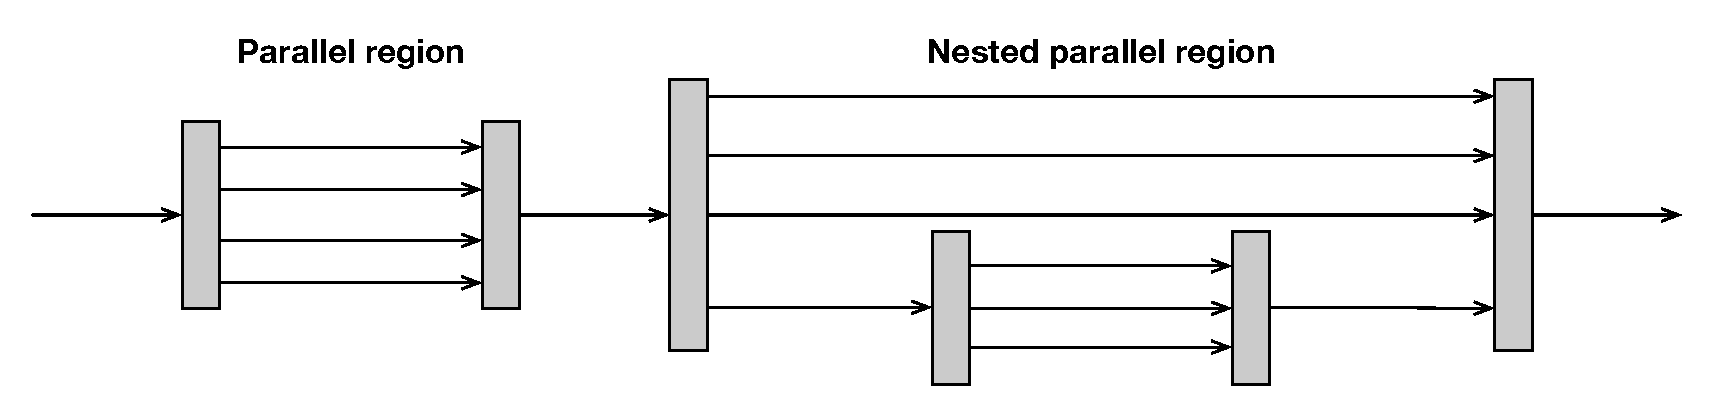
\includegraphics[width=0.95\textwidth]{figures/nested_parallelism}
  \caption{OpenMP nested parallelism}
  \label{fig:nested}
\end{figure}

\begin{itemize}
\item Static + dynamic analysis
\item Sequential blacklisting due to OpenMP structured parallelism
\item Barrier intervals
\item labeling to identify concurrent threads
\item sort of lock-set
\item Implemented by central but fast data structure
\item OMPT/OMPD
\end{itemize}

%%% Local Variables:
%%% mode: latex
%%% eval: (flyspell-mode 1)
%%% TeX-master: "root.tex"
%%% End:
